%%%%%%%%%%%%%%%%%%%%%%%%%%%%%%%%%%%%%%%%%
% Tufte-Style Book (Documentation Template)
% LaTeX Template
% Version 1.0 (5/1/13)
%
% This template has been downloaded from:
% http://www.LaTeXTemplates.com
%
% Original author:
% The Tufte-LaTeX Developers (tufte-latex.googlecode.com)
%
% License:
% Apache License (Version 2.0)
%
% IMPORTANT NOTE:
% In addition to running BibTeX to compile the reference list from the .bib
% file, you will need to run MakeIndex to compile the index at the end of the
% document.
%
%%%%%%%%%%%%%%%%%%%%%%%%%%%%%%%%%%%%%%%%%

%----------------------------------------------------------------------------------------
%	PACKAGES AND OTHER DOCUMENT CONFIGURATIONS
%----------------------------------------------------------------------------------------

\documentclass{tufte-book} % Use the tufte-book class which in turn uses the tufte-common class

\hypersetup{colorlinks} % Comment this line if you don't wish to have colored links

\usepackage{microtype} % Improves character and word spacing

\usepackage{lipsum} % Inserts dummy text

\usepackage{booktabs} % Better horizontal rules in tables

\usepackage{graphicx} % Needed to insert images into the document
\graphicspath{{graphics/}} % Sets the default location of pictures
\setkeys{Gin}{width=\linewidth,totalheight=\textheight,keepaspectratio} % Improves figure scaling

\usepackage{fancyvrb} % Allows customization of verbatim environments
\fvset{fontsize=\normalsize} % The font size of all verbatim text can be changed here

\newcommand{\hangp}[1]{\makebox[0pt][r]{(}#1\makebox[0pt][l]{)}} % New command to create parentheses around text in tables which take up no horizontal space - this improves column spacing
\newcommand{\hangstar}{\makebox[0pt][l]{*}} % New command to create asterisks in tables which take up no horizontal space - this improves column spacing

\usepackage{xspace} % Used for printing a trailing space better than using a tilde (~) using the \xspace command

\newcommand{\monthyear}{\ifcase\month\or January\or February\or March\or April\or May\or June\or July\or August\or September\or October\or November\or December\fi\space\number\year} % A command to print the current month and year

\newcommand{\openepigraph}[2]{ % This block sets up a command for printing an epigraph with 2 arguments - the quote and the author
\begin{fullwidth}
\sffamily\large
\begin{doublespace}
\noindent\allcaps{#1}\\ % The quote
\noindent\allcaps{#2} % The author
\end{doublespace}
\end{fullwidth}
}

\newcommand{\blankpage}{\newpage\hbox{}\thispagestyle{empty}\newpage} % Command to insert a blank page

\usepackage{units} % Used for printing standard units

\newcommand{\hlred}[1]{\textcolor{Maroon}{#1}} % Print text in maroon
\newcommand{\hangleft}[1]{\makebox[0pt][r]{#1}} % Used for printing commands in the index, moves the slash left so the command name aligns with the rest of the text in the index 
\newcommand{\hairsp}{\hspace{1pt}} % Command to print a very short space
\newcommand{\ie}{\textit{i.\hairsp{}e.}\xspace} % Command to print i.e.
\newcommand{\eg}{\textit{e.\hairsp{}g.}\xspace} % Command to print e.g.
\newcommand{\na}{\quad--} % Used in tables for N/A cells
\newcommand{\measure}[3]{#1/#2$\times$\unit[#3]{pc}} % Typesets the font size, leading, and measure in the form of: 10/12x26 pc.
\newcommand{\tuftebs}{\symbol{'134}} % Command to print a backslash in tt type in OT1/T1

\providecommand{\XeLaTeX}{X\lower.5ex\hbox{\kern-0.15em\reflectbox{E}}\kern-0.1em\LaTeX}
\newcommand{\tXeLaTeX}{\XeLaTeX\index{XeLaTeX@\protect\XeLaTeX}} % Command to print the XeLaTeX logo while simultaneously adding the position to the index

\newcommand{\doccmdnoindex}[2][]{\texttt{\tuftebs#2}} % Command to print a command in texttt with a backslash of tt type without inserting the command into the index

\newcommand{\doccmddef}[2][]{\hlred{\texttt{\tuftebs#2}}\label{cmd:#2}\ifthenelse{\isempty{#1}} % Command to define a command in red and add it to the index
{ % If no package is specified, add the command to the index
\index{#2 command@\protect\hangleft{\texttt{\tuftebs}}\texttt{#2}}% Command name
}
{ % If a package is also specified as a second argument, add the command and package to the index
\index{#2 command@\protect\hangleft{\texttt{\tuftebs}}\texttt{#2} (\texttt{#1} package)}% Command name
\index{#1 package@\texttt{#1} package}\index{packages!#1@\texttt{#1}}% Package name
}}

\newcommand{\doccmd}[2][]{% Command to define a command and add it to the index
\texttt{\tuftebs#2}%
\ifthenelse{\isempty{#1}}% If no package is specified, add the command to the index
{%
\index{#2 command@\protect\hangleft{\texttt{\tuftebs}}\texttt{#2}}% Command name
}
{%
\index{#2 command@\protect\hangleft{\texttt{\tuftebs}}\texttt{#2} (\texttt{#1} package)}% Command name
\index{#1 package@\texttt{#1} package}\index{packages!#1@\texttt{#1}}% Package name
}}

% A bunch of new commands to print commands, arguments, environments, classes, etc within the text using the correct formatting
\newcommand{\docopt}[1]{\ensuremath{\langle}\textrm{\textit{#1}}\ensuremath{\rangle}}
\newcommand{\docarg}[1]{\textrm{\textit{#1}}}
\newenvironment{docspec}{\begin{quotation}\ttfamily\parskip0pt\parindent0pt\ignorespaces}{\end{quotation}}
\newcommand{\docenv}[1]{\texttt{#1}\index{#1 environment@\texttt{#1} environment}\index{environments!#1@\texttt{#1}}}
\newcommand{\docenvdef}[1]{\hlred{\texttt{#1}}\label{env:#1}\index{#1 environment@\texttt{#1} environment}\index{environments!#1@\texttt{#1}}}
\newcommand{\docpkg}[1]{\texttt{#1}\index{#1 package@\texttt{#1} package}\index{packages!#1@\texttt{#1}}}
\newcommand{\doccls}[1]{\texttt{#1}}
\newcommand{\docclsopt}[1]{\texttt{#1}\index{#1 class option@\texttt{#1} class option}\index{class options!#1@\texttt{#1}}}
\newcommand{\docclsoptdef}[1]{\hlred{\texttt{#1}}\label{clsopt:#1}\index{#1 class option@\texttt{#1} class option}\index{class options!#1@\texttt{#1}}}
\newcommand{\docmsg}[2]{\bigskip\begin{fullwidth}\noindent\ttfamily#1\end{fullwidth}\medskip\par\noindent#2}
\newcommand{\docfilehook}[2]{\texttt{#1}\index{file hooks!#2}\index{#1@\texttt{#1}}}
\newcommand{\doccounter}[1]{\texttt{#1}\index{#1 counter@\texttt{#1} counter}}

\usepackage{makeidx} % Used to generate the index
\makeindex % Generate the index which is printed at the end of the document

% This block contains a number of shortcuts used throughout the book
\newcommand{\vdqi}{\textit{VDQI}\xspace}
\newcommand{\ei}{\textit{EI}\xspace}
\newcommand{\ve}{\textit{VE}\xspace}
\newcommand{\be}{\textit{BE}\xspace}
\newcommand{\VDQI}{\textit{The Visual Display of Quantitative Information}\xspace}
\newcommand{\EI}{\textit{Envisioning Information}\xspace}
\newcommand{\VE}{\textit{Visual Explanations}\xspace}
\newcommand{\BE}{\textit{Beautiful Evidence}\xspace}
\newcommand{\TL}{Tufte-\LaTeX\xspace}
\usepackage{amssymb}
\usepackage{latexsym}
\usepackage{amsmath}
\usepackage{amsthm}
%\usepackage{stmaryrd}
\newcommand{\Swarrow}{\mathbin{\rotatebox[origin=c]{45}{$\Leftarrow$}}}
\usepackage{fancyhdr}
\pagestyle{headings}
\usepackage{dsfont}
\usepackage{pifont}
\usepackage{mathtools}
\usepackage{natbib}
\usepackage{tikz-cd}
\usepackage{pgfplots}
\usepackage{enumitem}
\tikzset{
  subseteq/.style={
    draw=none,
    edge node={node [sloped, allow upside down, auto=false]{$\subseteq$}}
    },
  Subseteq/.style={
    draw=none,
    every to/.append style={
      edge node={node [sloped, allow upside down, auto=false]{$\subseteq$}}}
    },
    Subsetneq/.style={
    draw=none,
    every to/.append style={
      edge node={node [sloped, allow upside down, auto=false]{$\subsetneq$}}}
    },
  Supseteq/.style={
    draw=none,
    every to/.append style={
      edge node={node [sloped, allow upside down, auto=false]{$\supseteq$}}}
  }
}
\newcounter{dummy} 
\numberwithin{dummy}{section}
\newtheorem{thm}{Theorem}[dummy]
\newtheorem{prop}[thm]{Proposition}
\newtheorem{lemma}[thm]{Lemma}
\newtheorem{cor}[thm]{Corollary}
\newtheorem{dfn}[thm]{Definition}
\newtheorem{axiom}[thm]{Axiom}
\newtheorem{rmk}[thm]{Remark}
\newtheorem{rmkt}[thm]{Remark by TeXer}
\newtheorem{ex}[thm]{Example}
\newtheorem{nex}[thm]{Non-example}
\newtheorem{exercise}[thm]{Exercise}
\newtheorem{question}[thm]{Question}
\newtheorem{problem}[thm]{Problem}
\newtheorem{dfn/thm}[thm]{Definition/Theorem}
\renewcommand*{\thethm}{\thesection.\arabic{thm}}

%------------------------Colors----------------------------
\definecolor{mygray}{gray}{0.6}

%-------------------------Short cuts----------------------
\renewcommand{\baselinestretch}{1.1}
\newcommand{\mor}{{\textnormal Mor\,}}
\renewcommand{\hom}{{\textnormal Hom}}
\newcommand{\reals}{\mathbb R}
\newcommand{\cplx}{\mathbb C}
\newcommand{\intg}{\mathbb Z}
\newcommand{\bbf}{\mathbb F}
\newcommand{\ratl}{\mathbb Q}
\newcommand{\torus}{\mathbb T}
\newcommand{\sca}{{\mathfrak a}}
\newcommand{\scb}{{\mathfrak b}}
\newcommand{\scc}{{\mathfrak c}}
\newcommand{\scm}{{\mathfrak m}}
\newcommand{\scn}{{\mathfrak n}}
\newcommand{\scp}{{\mathfrak p}}
\newcommand{\scq}{\mathfrak q}
\newcommand{\frakg}{{\mathfrak g}}
\newcommand{\frakd}{{\mathfrak d}}
\newcommand{\pd}{{\partial}}
\newcommand{\calf}{{\cal F}}
\newcommand{\calg}{{\cal G}}
\newcommand{\cala}{{\cal A}}
\newcommand{\calb}{{\cal B}}
\newcommand{\calc}{{\cal C}}
\newcommand{\cald}{{\cal D}}
\newcommand{\cale}{{\cal E}}
\newcommand{\cali}{{\cal I}}
\newcommand{\call}{{\cal L}}
\newcommand{\calm}{{\cal M}}
\newcommand{\caln}{{\cal N}}
\newcommand{\calo}{{\cal O}}
\newcommand{\calr}{{\cal R}}
%\newcommand{\mathbold}{\bf}
\newcommand{\cinf}{C^{\infty}}
\newcommand{\row}[2]{#1_1,\dots ,#1_{#2}}
\newcommand{\dbyd}[2]{{\partial #1\over\partial #2}}
\newcommand{\Space}{{\bf Space}}
\newcommand{\alg}{{\mathbold Alg}}
\newcommand{\notsubset}{\not \subset}
\newcommand{\notsupset}{\not \supset}
\newcommand{\pois}{{\mathbold Pois}}
\newcommand{\pitilde}{\tilde{\pi}}
\newcommand{\rta}{\rightarrow}
\newcommand{\llta}{\longleftarrow}
\newcommand{\Lrta}{\Longrightarrow}
\newcommand{\lrta}{\longrightarrow}
\newcommand{\llrta}{\longleftrightarrow}
\newcommand{\Llta}{\Longleftarrow}
\newcommand{\Llrta}{\Longleftrightarrow}
\newcommand{\lgl}{\langle}
\newcommand{\rgl}{\rangle}
\newcommand{\inj}{\hookrightarrow}
\newcommand{\surj}{\twoheadrightarrow}
\newcommand{\cmark}{\ding{51}}%
\newcommand{\xmark}{\ding{55}}%
\newcommand{\downmapsto}{\rotatebox[origin=c]{-90}{$\scriptstyle\mapsto$}\mkern2mu}
\renewcommand{\qedsymbol}{$\square$}
\newcommand{\ssh}{\mathsf{Sh}}
\newcommand{\bfp}{\mathbf{P}}
%----------------------------------------------------------------------------------------
%	BOOK META-INFORMATION
%----------------------------------------------------------------------------------------

\title{Mastere course on algebraic stacks} % Title of the book

\author{French version by Bertrand Toen\\
Translated by Lind Axiao} % Author

%\publisher{Publisher of This Book} % Publisher

%----------------------------------------------------------------------------------------

\begin{document}

\frontmatter

%----------------------------------------------------------------------------------------
%	EPIGRAPH
%----------------------------------------------------------------------------------------

%\thispagestyle{empty}
%\openepigraph{The public is more familiar with bad design than good design. It is, in effect, conditioned to prefer bad design, because that is what it lives with. The new becomes threatening, the old reassuring.}{Paul Rand, {\itshape Design, Form, and Chaos}}
%\vfill
%\openepigraph{A designer knows that he has achieved perfection not when there is nothing left to add, but when there is nothing left to take away.}{Antoine de Saint-Exup\'{e}ry}
%\vfill
%\openepigraph{\ldots the designer of a new system must not only be the implementor and the first large-scale user; the designer should also write the first user manual\ldots If I had not participated fully in all these activities, literally hundreds of improvements would never have been made, because I would never have thought of them or perceived why they were important.}{Donald E. Knuth}

%----------------------------------------------------------------------------------------

\maketitle % Print the title page

%----------------------------------------------------------------------------------------
%	COPYRIGHT PAGE
%----------------------------------------------------------------------------------------

\newpage
\begin{fullwidth}
~\vfill
\thispagestyle{empty}
\setlength{\parindent}{0pt}
\setlength{\parskip}{\baselineskip}
Copyright \copyright\ \the\year\ \thanklessauthor

\par\smallcaps{Published by \thanklesspublisher}

\par\smallcaps{tufte-latex.googlecode.com}

\par Licensed under the Apache License, Version 2.0 (the ``License''); you may not use this file except in compliance with the License. You may obtain a copy of the License at \url{http://www.apache.org/licenses/LICENSE-2.0}. Unless required by applicable law or agreed to in writing, software distributed under the License is distributed on an \smallcaps{``AS IS'' BASIS, WITHOUT WARRANTIES OR CONDITIONS OF ANY KIND}, either express or implied. See the License for the specific language governing permissions and limitations under the License.\index{license}

\par\textit{First printing, \monthyear}
\end{fullwidth}

%----------------------------------------------------------------------------------------

\tableofcontents % Print the table of contents

%----------------------------------------------------------------------------------------

%\listoffigures % Print a list of figures

%----------------------------------------------------------------------------------------

%\listoftables % Print a list of tables

%----------------------------------------------------------------------------------------
%	DEDICATION PAGE
%----------------------------------------------------------------------------------------

%\cleardoublepage
%~\vfill
%\begin{doublespace}
%\noindent\fontsize{18}{22}\selectfont\itshape
%\nohyphenation
%Dedicated to those who appreciate \LaTeX{} and the work of \mbox{Edward R.~Tufte} and %\mbox{Donald E.~Knuth}.
%\end{doublespace}
%\vfill
%\vfill

%----------------------------------------------------------------------------------------
%	INTRODUCTION
%----------------------------------------------------------------------------------------

\cleardoublepage
\chapter{Introduction} % The asterisk leaves out this chapter from the table of contents

This sample book discusses the design of Edward Tufte's books\cite{Tufte2001,Tufte1990,Tufte1997,Tufte2006} and the use of the \doccls{tufte-book} and \doccls{tufte-handout} document classes.

%----------------------------------------------------------------------------------------

\mainmatter

%----------------------------------------------------------------------------------------
%	CHAPTER 1
%----------------------------------------------------------------------------------------
\chapter{Reflections on the notion of space}
\section{Lecture 1: Reflections on the notion of space I}
The goal of the first course is to understand the notion of manifold in different contexts (topological, differentiable, analytic...) We will start by looking at the case of topological manifolds.
\subsection*{Reminders on topological manifolds}
\begin{dfn}
\begin{enumerate}
  \item A \textbf{topological manifold} is a topological space $X$, which has an open cover $\{U_i\}_{i\in I}$ such that for each $i\in I$, there exists a homeomorphism between $U_i$ and an open subset in $\reals^{n_i}$ 

  \item the category of topological manifold is a subcategory of $\mathsf{Top}$. It is denoted as $\mathsf{VarTop}$. 
\end{enumerate}
\end{dfn}

Let $X$ be a topological manifold and $\{U_i\}_{i\in I}$ is an open cover as in the definition above. We put, for $i$ and $j$ in $I$, $U_{i,j}:=U_i\cap U_j$. We have a diagram of topological spaces
$$
\coprod_{(i,j)\in I^2}U_{i,j}\rightrightarrows \coprod_{i\in I} U_{i},
$$
where the first morphism sends the component $U_{i,j}$ into $U_i$ by the inclusion $U_{i,j}\inj U_i$, and the second morphism sends $U_{i,j}$ into $U_j$ by the inclusion $U_{i,j}\inj U_j$. There also exists  a morphism
$$
\coprod_{i\in I} U_i\lrta X
$$
which restricts to inclusion $U_i\inj X$ for all $i$, which equalizes the above two morphisms. We obtain also a well-defined morphism from the coequalizer of the first diagram to $X$
$$
\text{Colim}\left(\coprod_{(i,j)\in I^2}U_{i,j}\rightrightarrows \coprod_{i\in I}U_i\right)\lrta X.
$$
What makes it important is the following lemma.
\begin{lemma}
The morphism 
$$
\textnormal{Colim}\left(\coprod_{(i,j)\in I^2}U_{i,j}\rightrightarrows \coprod_{i\in I}U_i\right)\lrta X
$$
is an isomorphism.
\end{lemma}
\begin{proof}
The lemma says that for a topological space $Y$, and a given morphism $f:X\lrta Y$ is the same as giving for each $i\in I$ a morphism $f_i:U_i\lrta Y$ so that $(f_i)|_{U_{i,j}}=(f_j)|_{U_{i,j}}$ for all $(i,j)\in I^2$. (This is a direct translation of the universal property of the coequalizer. Which is true by the gluing lemma of continuous maps)
\end{proof}
The above lemma has to be interpreted in the following way: all topological manifold is obtained from a colimit of a diagram of open sets in $\reals^n$ (for $n$ variable). we can draw from it the following principle:

\textit{The category $\mathsf{TopMfd}$ of the topological manifolds can be constructed from the category of open sets in $\reals^n$ (with morphism continuous maps).}

We would explain the principle in the following section.
\subsection{Manifold and sheaves}
Let $\calc$ be the full subcategory of $\mathsf{TopMfd}$, of which the objects are open sets in $\reals^n$ for some $n$. We denote $\mathsf{Pr}(\calc)$ the category of presheaves of sets on $\calc$, (also denoted as $\widehat{\calc}$ ). We consider Yoneda embedding in the case of $\calc$
$$
\begin{aligned}
h\_: \mathsf{TopMfd}&\lrta \mathsf{Pr}(\calc)\\
X&\longmapsto h_X,
\end{aligned}
$$
where the presheaf $h_X$ is defined by 
$$
h_X(Y):=\hom_{\mathsf{TopMfd}}(Y,X)
$$
for all $Y\in \calc\subset \mathsf{TopMfd}$.

\begin{lemma}\label{lem:yoneda_full_faithful}
The functor $h\_$ above is full and faithful.
\end{lemma}
\begin{proof}
The functor is faithful: for two morphisms $f,g:X\lrta X'$, we consider an open cover $\{U_i\}$ of $X$ so that each $U_i\in\calc$ this exists because $X$ is a manifold). If $h_f=h_g$, for every $i\in I$, the two maps 
$$
h_f(U_i)=h_g(U_i):\hom(U_i, X)=h_X(U_i)\lrta \hom(U_i, X')=h_{X'}(U_i)
$$
are equal. This means that $f|_{U_i}=g|_{U_i}$, for every $i$, hence that $f=g$. 

The functor is full: Let $X$ and $X'$ be two topological manifolds and $u:h_X\lrta h_{X'}$ is a morphism of in $\mathsf{Pr}(\calc)$. Let $\{U_i\}$ be an open cover of $X$ with $U_i\in \calc$. For all $i$, the morphism $u$ induces a map 
$$
h_X(U_i)=\hom(U_i,X)\lrta h_{X'}(U_i)=\hom(U_i,X').
$$
This map send the 
inclusion $U_i\subset X$ to morphisms $f_i:U_i\lrta X'$ for all $i$.  For all $i$ and $j$ in $I$, the elements $(f_i)|_{U_{i,j}}\in h_{X'}(U_{i,j})$ agree because they are both images of the inclusion $U_{i,j}\inj X$ because the morphism of presheaves $u$ is compatible with the restriction maps. There the morphisms $f_i:U_i\lrta X'$ give a continuous map $f:X\lrta X'$. By construction $h_f=u$.
\end{proof}
The Lemma~\ref{lem:yoneda_full_faithful} is a good point remark, we know $\mathsf{TopMfd}$ can be identified with a full subcategory of $\mathsf{Pr}(\calc)$. We are now seeking to characterize the subcategory.

We start by making $\calc$ a Grothendieck site. We say a collection of morphism $\{U_i\lrta U\}_{i\in I}$ in $\calc$ is a \textbf{covering family} if each morphism $U_i\lrta U$ is an open immersion and if the map $\coprod_{i\in I}U_i\lrta U$ is surjective. This define a pretopology on $\calc$ (Exercise, verify this\sidenote{Check the covering family defined above satisfies \href{https://ncatlab.org/nlab/show/Grothendieck+pretopology}{the axioms} of Grothendieck pretopology. And the Grothendieck topology $\tau$ on $\calc$ is generated by union of covering families (or, the covering family gives a basis of topology $\tau$)}), and we denote the associated topology $\tau$. 
\begin{lemma}\label{lem:sheaf_on_site}
For all $X\in \mathsf{TopMfd}$ the presheaf $h_X\in\mathsf{Pr}(\calc)$ is a sheaf with respect to the topology $\tau$.
\end{lemma}
\begin{proof}
See the \href{https://stacks.math.columbia.edu/tag/00VM}{definition} of a sheaf on a site.
It is another way of saying for each topological manifold $Y$ and an open cover $\{U_i\lrta Y\}_{i\in I}$, to give a continuous map from $Y$ to $X$ is the same as to give a a collection of continuous map $f_i:U_i\lrta X$ such that $f_i$ and $f_j$ coincide on $U_i\cap U_j$. 
\end{proof}
As a result, the Lemma~\ref{lem:sheaf_on_site} implies that the there is a fully faithful functor 
$$
h\_: \mathsf{TopMfd}\lrta\mathsf{Sh}(\calc,\tau).
$$
A sheaf isomorphic to $h_X$ is called \textbf{representable} by $X$. In a general way, we identify the category of $\mathsf{TopMfd}$ with its image in $\mathsf{Sh}(\calc,\tau)$.

To characterize the image, we put the following definition
\begin{dfn}\label{dfn:local_homeomorphism_open_immersion}\ 
\begin{enumerate}
\item A morphism $f: F\lrta G$ in $\mathsf{Sh}(\calc,\tau)$ is a \textbf{local homeomorphism} if for all $X\in\calc$ and each morphism $h_X\lrta G$, the sheaf $F\times_G h_X$ is representable by $Y\in \mathsf{TopMfd}$, and the induced morphism $Y\lrta X$ by the projection $F\times_G h_X\simeq h_Y\lrta h_X$ is a local homeomorphism as morphism in $\mathsf{Top}$. 
\item A morphism in $\mathsf{Sh}(\calc,\tau) $ is an \textbf{open immersion} if it is a monomorphism and a local homeomorphism.
\end{enumerate}
\end{dfn}
It is easy to check that the open immersions in $\mathsf{Sh}(\calc,\tau)$ are stable under composition. We can also verify that the local homeomorphisms  are stable under composition, but it requires corollary~\ref{cor:criterion_representable} below. We also show that a morphism of topological manifolds $X\lrta Y$ is a local homeomorphism of topological spaces if and only if the morphism of sheaves $h_X\lrta h_Y$ is a local homeomorphism as defined above.

We therefore have the proposition below.
\begin{prop}\label{lem:criterion_representable_TopMfd}
A sheaf $F\in \mathsf{Sh}(\calc,\tau)$ is representable by one topological manifold iff there exists a family of objects $\{U_i\}_{i\in I}$ in $\calc$, and a morphism of sheaves
$$
p:\coprod_{i\in I}h_{U_i}\lrta F,
$$ 
that satisfy the following two conditions
\begin{enumerate}
\item The morphism $p$ is an epimorphism of sheaves.
\item For each $i\in I$, the morphism $h_{U_i}\lrta F$ is an open immersion.
\end{enumerate}
\end{prop} 
\begin{proof}
We start by supposing that $F$ is representable by one topological manifold $X$. We choose an open cover $\{U_i\}_{i\in I}$ of $X$ with $U_i\in \calc$ and we consider the morphism
$$
p:\coprod_{i\in I}h_{U_i}\lrta F\simeq h_X
$$
induced by the inclusion $U_i\subset X$. Explicitly, we have
$$
p(W):\left(\coprod_{i}h_{U_i}\right)(W)=\coprod_i h_{U_i}(W)\lrta h_X(W).
$$ 
For $Y\in \calc$ and $f:Y\lrta X$ an element in $h_X(Y)=\hom(Y,X)$, we regard $\{f^{-1}(U_i)\}_{i\in I}$ as an open cover of $Y$. Furthermore, for each $i\in I$, there exists a commutative diagram
$$
\begin{tikzcd}
f^{-1}(U_i) \arrow[d,"g"] \arrow[r] & Y \arrow[d,"f"] \\
U_i \arrow[r] & X
\end{tikzcd}
$$
which show that $f$ is locally in the image of $p$ in the sense that $f|_{f^{-1}(U_i)}$ is in the image of $p(U_i)$. By \href{http://stacks.math.columbia.edu/tag/00WL}{Tag 00WL, stacks-project},  this implies that $p$ is an epimorphism of sheaves. Moreover, for $Y\in \calc$ and for all morphism $h_Y\lrta h_X$, corresponding to a morphism $f:Y\lrta X$, we have
$$
h_{U_i}\times_{h_{X}}h_Y\simeq h_{U_i\times_X Y}=h_{f^{-1}(U_i)},
$$
where the induced map $f^{-1}(U_i)\lrta Y$ is the plain inclusion hence must be local homeomorphism in $\mathsf{Top}$,
which means $h_{U_i}\lrta F$ is a local homeomorphism by definition.
As $f^{-1}(U_i)\lrta Y$ is an open immersion, we observe that every morphism $h_{U_i}\lrta F$ is an open immersion. ($h$ is fully faithful, therefore preserves limits and colimits, thus gives us the equality above. For the same reason $h$ preserves monomorphisms, hence $h_{f^{-1}(U_i)}\lrta h_Y$ is a monomorphism. Take the special case $Y=X$, $h_{U_i}\lrta F$ is a monomorphism.)

Conversely, suppose $F$ is a sheaf satisfying the two conditions in the proposition. We construct the topological space $X$ in the following way: let $\{U_i\}_{i\in I}$ be a family of objects in the category $\calc$ and $p:\coprod h_{U_i}\lrta F$ is a morphism in the statement of the proposition. We set $U=\coprod_i U_i\in \mathsf{TopMfd}$. We remark that the morphism
$$
\coprod h_{U_i}\lrta h_U
$$
is an isomorphism in $\mathsf{Sh}(\calc,\tau)$ (Exercise, verify this.) We consider the two projections
$$
h_U\times_F h_U\rightrightarrows h_U.
$$
By hypothesis, we have
$$
h_U\times_F h_U= \coprod_{i} h_{U_i}\times_F\coprod_{j} h_{U_j}\simeq\coprod_{i,j} h_{U_{i,j}}\simeq h_R,
$$
where $R=\coprod_{i,j}U_{i,j}$, with $h_{U_{i,j}}\simeq h_{U_i}\times_F h_{U_j}$. ($U_{i,j}$ is the representing object of $h_{U_i}\times_F h_{U_j}$, is isomorphic to an open set in $U_i$ and in $U_j$). The second isomorphism above is from the fact that finite limit commutes with filtered colimit. By Lemma~\ref{lem:yoneda_full_faithful} and Lemma~\ref{lem:sheaf_on_site} the diagram 
$$
h_R\rightrightarrows h_U
$$
is image by $h$ of the diagram of topological manifolds $R\rightrightarrows U$. We set the 
$$
X:=\textnormal{colim}(R\rightrightarrows U),
$$
where the colimit is taken in the category $\mathsf{Top}$. Note that $R$ defines an equivalence relation on $U$ and that $X$ is the quotient space.

We further remark that $X$ is a topological manifold. For it, observe by definition the morphism $U\lrta X$ is surjective. More over, $U_i\lrta X$ is an open immersion. Indeed, from the fact that $h_{U_i}\lrta F$ is a monomorphism , we have $U_{i,i}=U_i$, which implies that $U_i\lrta X$ is injective (Exercise, verify this
\sidenote{
  {
  \color{gray}
  \begin{proof}[sol]
  ada
  \end{proof}
  }
}
). Moreover, a subset $V\subset X$ is open iff its preimage in $U$ by the projection $U\lrta X$ is open. But the inverse image of $U_i\subset X$ by the projection is the subset $\coprod_j U_{i,j}\subset U$ which is indeed an open set. This shows that $X$ is covered by the opens $U_i\in\calc$, and therefore is a topological manifold.

It remains to show that $F$ is isomorphic to $h_X$. There exists a morphism of sheaves
$$
\textnormal{colim}(h_R\rightrightarrows h_U)\lrta h_X.
$$
Because $h_U\lrta F$ is an epimorphism and that the epimorphism of sheaves are \href{https://ncatlab.org/nlab/show/effective+epimorphism}{  effective epimorphisms}.
\sidenote{{\color{red} References needed}}
By the definition of effective epimorphism
$$
\textnormal{colimit}(h_U\times_Fh_U\rightrightarrows h_U)\simeq F
$$
and because $h_R\simeq h_U\times_F h_U$ as described above, we have
$$
F\simeq \textnormal{colimit}(h_R\rightrightarrows h_U).
$$
It then remains verify that $\textnormal{colim}(h_R\rightrightarrows h_U)\simeq h_X$. $h_U\lrta h_X$ is also an epimorphism of sheaves (Exercise, verify this), it remains to show that the morphism
$$
h_R\lrta h_U\times_{h_X} h_U
$$
is an isomorphism.

Recall that $h$ is a fully faithful functor, it suffices to verify that the morphism
$$
R\lrta U\times_X U
$$ is an isomorphism, which is true because the morphism $U_{i,j}\lrta U_i\times_X U_j$ is an isomorphism. (It is bijective local homeomorphism\sidenote[][-3\baselineskip]{{\color{gray}
Explicitly, $U_i\times_X U_j=\{(u,v)\in U_i\coprod U_j: \iota_i(u)=\iota_j(v)\}$}})
\begin{marginfigure}[-4\baselineskip]
{\color{gray}
$$
\tiny
\begin{tikzcd}
U_{i,j} \arrow[rdd, "\alpha_{i,j}"'] \arrow[rrd, "\beta_{i,j}"] \arrow[rd, dashed] &  &  \\
 & U_i\times_X U_j \arrow[d] \arrow[r] & U_j \arrow[d, "\iota_j"] \\
 & U_i \arrow[r, "\iota_i"'] & X
\end{tikzcd}
$$
%\caption*{This is a margin figure. The helix is defined by $x = \cos(2\pi z)$, $y = \sin(2\pi z)$, and $z = [0, 2.7]$. The figure was drawn using Asymptote (\url{http://asymptote.sf.net/}).}
\label{fig:marginfig}
the dashed arrow is given by $z\longmapsto (\alpha_{i,j}(z),\beta_{i,j}(z))$, it is injective because $\alpha_{i,j},\beta_{i,j}$ are injective. It is surjective because $X:=\coprod_i U_i/\sim$, where $\iota_i(u)=\iota_j(v)$ iff
$(u,v)=(\alpha_{i,j}(z),\beta_{i,j}(z))$ for some $z\in U_{i,j}$. And by hypothesis, $h_{U_i}\lrta F$ is open immersion therefore is a local homeomorphism, we know $\alpha_{i,j},\beta_{i,j}$ are local homeomorphism. Altogether we know $z\mapsto (\alpha_{i,j}(z),\beta_{i,j}(z))$ is a bijective local homeomorphism hence a homeomorphism.
}
\end{marginfigure}
\end{proof}
\begin{cor}\label{cor:criterion_representable}
Let $X\in\mathsf{TopMfd}$, and $F\lrta h_X$ a morphism of sheaves. If there exists an open covering $\{U_i\}_{i\in I}$ of $X$ so that for all $i\in I$ the sheaf $F\times_{h_X} h_{U_i}$ is representable by a topological manifold, the sheaf $F$ is representable by a topological manifold.
\end{cor}
\begin{proof}
For each $i\in I$, we choose $\{V_{i,j}\}_{j\in J}$ and $\coprod_j h_{V_{i,j}}\lrta F\times_{h_X} h_{U_i}$ from the above proposition~\ref{lem:criterion_representable_TopMfd}. We verify then
$$
\coprod_{i,j}h_{V_{i,j}}\lrta F
$$
is a morphism from the proposition~\ref{lem:criterion_representable_TopMfd}(Exercise, verify this)
\end{proof}
\subsection{Quotient manifolds}
Let $G$ be a group (discrete) that operate on the topological manifold $X\in \mathsf{TopMfd}$. By functoriality, the group $G$ acts on the sheaf $h_X$. Recall that the action $G$ on $X$ is free if for every $x\in X$ and $g\in G$, we have $(g\cdot x=x)\lrta (g=e)$. Recall also the that the action of group $G$ on $X$ is totally discontinuous if all point $x\in X$ has an open neighborhood $U\subset X$ so that for all $g\in G$ we have
$$
(g(U)\cap U\neq \emptyset)\Lrta (g=e).
$$

In the following statement, we should take care not to confuse the quotient sheaf $h_X/G$ and the sheaf $h_{X/G}$ represented by the quotient topological manifold $X/G$.

\begin{prop}\label{prop:quotient_group_action}
\ \begin{enumerate}
\item If the action of the group $G$ on $X$ is free, then the quotient morphism 
$$
h_X\lrta h_X/G
$$
is a local homeomorphism.
\item If the group action $G$ on $X$ is totally discontinuous, then sheaf quotient $h_X/G\in \mathsf{Sh}(\calc,\tau)$ is representable by a topological manifold.
\end{enumerate}
\end{prop}
\begin{proof}
(1) Let $Y\in \calc$ and $h_Y\lrta h_X/G$ be a morphism of sheaves. We must firstly show that $h_X\times_{h_X/G}h_Y$ is  a topological manifold. Since the quotient morphism $h_X\lrta h_X/G$ is an epimorphism, there exists an open cover $\{Y_i\}$ of $Y$ and the the following diagram commutes\sidenote[][-6\baselineskip]{{\color{gray} Denote the natural transformation $\eta:h_X\lrta h_X/G$
$id_Y$ maps to equivalence class $[\eta(id_Y)]\in h_{X}/G(Y)$ and we can choose one element $f\in [\eta(id_Y)]$. Recall the stability axiom of Grothendieck pretopology, the pull back of the covering family $\{X_i\lrta X\}$ gives a covering family $\{Y_i:=f^*X_i\lrta X\}$of $Y$} }
$$
\begin{tikzcd}
\coprod_i h_{Y_i} \arrow[d] \arrow[r] & h_Y \arrow[d] \\
h_X \arrow[r] & h_X/G.
\end{tikzcd}
$$
Apply the Corollary~\ref{cor:criterion_representable} to the morphism
$$
h_X\times_{h_X/G}h_Y\lrta h_Y.
$$
It suffices to show that each $h_X\times_{h_X/G}h_{Y_i}$ is representable by a topological manifold.\sidenote[][-6\baselineskip]{{\color{gray}
The Corollary~\ref{cor:criterion_representable} says given $F\lrta h_Z$ and $Z\in\mathsf{TopMfd}$, $F$ is representable if $Y\in \mathsf{TopMfd}$ and each $F\times_{h_Z}h_{Y_i}$ is representable. This is automatically implied if we can prove the representability of $h_X\times_{h_X/G}h_{Y_i}$ for the general case $Y\in\calc$.
}}Note that we also have the composition of pushout
$$
h_X\times_{h_X/G}h_{Y_i}\simeq (h_X\times_{h_X/G}h_X)\times_{h_X}h_{Y_i}.
$$
Now, $h_X\times_{h_X/G}h_X\simeq h_X\times h_G$ as can be verified  at the level of presheaves of sets (Exercise, verify this\sidenote[][]{aaaa}). Thus, we have
$$
h_X\times_{h_X.G}h_{Y_i}\simeq h_{Y_i}\times h_G\simeq h_{Y_i\times G}.
$$
$Y_i\times G\in \mathsf{TopMfd}$, which finishes the proof that $h_X\times_{h_X/G}h_Y$ is representable by a topological manifold. Moreover, the morphism of manifolds
$$
h_X\times_{h_X/G}h_Y\lrta h_Y
$$
is, after restricting to the cover $\{Y_i\}$, isomorphic to the projection
$$
h_{Y_i}\times h_G\lrta h_{Y_i}.
$$
It follows that the morphism is local homeomorphism in $\mathsf{Top}$, which implies the the morphism $h_X\lrta h_{X}/G$ is local homeomorphism in $\mathsf{TopMfd}$.

(2) For all $x\in X$ there is an open neighborhood $U_x$ of $x$ in $X$ so that $g(U_x)\cap U_x=\emptyset$ for all $g\neq e$ in $G$. We consider the morphism
$$
h_{U_x}\lrta h_X/G.
$$
By point $(1)$, the morphism is a composition of local homeomorphisms $(h_{U_x}\lrta h_X\lrta h_X/G)$ and therefore is a local homeomorphism. Moreover,  we have
$$
h_{U_x}\times_{h_X/G}h_{U_x}\simeq (h_{U_x}\times_{h_X/G}h_X)\times_{h_X}h_{U_x}\simeq (h_{U_x}\times h_G)\times_{h_X}h_{U_x},
$$
as we have seen before in the proof of point $(1)$. Finally, we have
$$
h_{U_x}\times h_G)\times_{h_X}h_{U_x}\simeq h_{(U_x\times G)\times_X U_x}.
$$
According to the choice of $U_x$, we have $(U_x\times G)\times_X U_x\simeq U_x$ (Exercise, verify this). Hence, we have shown that the morphism
$$
h_{U_x}\lrta h_{U_x}\times_{h_X/G}h_{U_x}
$$
is an isomorphism. Equivalently, the morphism
$$
h_{U_x}\lrta h_X/G
$$
is an monomorphism. This shows that for all $x\in X$ the morphism
$$
h_{U_x}\lrta h_X/G
$$
is an open immersion. Also recall that the total morphism
$$
\coprod_{x\in X}h_{U_x}\lrta h_X\lrta h_X/G
$$
is an epimorphism, which finishes the proof.
\end{proof}
The corollary above implies that the quotient $X/G$ also exists in the category $\mathsf{TopMfd}$ (because $h$ is fully faithful), but it is a stronger statement.
\subsection{Remarks on manifolds}
The Proposition~\ref{prop:quotient_group_action} provide a good method for us to construct topological manifold by totally discontinuous group actions, while the quotient topological space $X/G$ is in general very pathological. The sheaf quotient $h_X/G$ has better properties (e.g. point $(1)$ in Proposition~\ref{prop:quotient_group_action}), even if is no longer representable by topological manifold.

The following is a striking example: we make the discrete group $\ratl$ (for additive law) act on the topological space $\reals$ by the morphism
$$
\reals\times \ratl\lrta \reals
$$ 
by $(x,t)\longmapsto x+t$. It can be seen that the action is free, but not totally discontinuous. In addition, the morphism $\reals\lrta \reals/\ratl$ is not a local homeomorphism because it is not locally injective. In the end the quotient topology is given a ``gross'' topology (because the open sets in $\reals/\ratl$ is the invariant open set in $\reals$ under the group action). This shows that the quotient $\reals/\ratl$ is not a reasonable object from a geometric point of view. On the other hand, the quotient sheaf $h_\reals/\ratl$ seems more interesting, because the morphism $h_\reals\lrta h_\reals/\ratl$ being a local homeomorphism allow us to legally think about $h_\reals/\ratl$ as an open set in $\reals$ in a certain way. The sheaf $h_\reals/\ratl$ is the very first example of \textbf{geometric space}\sidenote{Is this the standard translation?}. 
\begin{dfn}
A sheaf $F\in\mathsf{Sh}(\calc,\tau)$ is a geometric space if there exists a family of objects $\{U_i\}_{i\in I}$ in $\calc$, and a morphism of sheaves
$$
p:\coprod_{i\in I}h_{U_i}\lrta F
$$
satisfying the following two conditions
\begin{enumerate}
\item The morphism $p$ is an epimorphism of sheaves.
\item For all $i\in I$ the morphism $h_{U_i}\lrta F$ is a local homeomorphism (in the sense of definition~\ref{dfn:local_homeomorphism_open_immersion}).
\end{enumerate}
\end{dfn}
The Proposition~\ref{prop:quotient_group_action} tells that the quotient sheaf $h_X/G$, for a free action of group $G$ on a topological manifold is a geometric space. An example of geometric space is $h_\reals/\ratl$ described above. Another example is $h_\reals/\intg+\alpha\intg$, where $\alpha\in \reals-\ratl$.

The geometric spaces form a full subcategory of $\mathsf{Sh}(\calc,\tau)$. This category will studied in detail the next lecture.

%------------------------------------------------
\section{Lecture 2: Reflections on the notion of space II}
In the last lecture, we have seen how the category of topological manifold can be reconstructed from the category $\calc$ of open sets in $\reals^n$. To be more precise, we have used the category $\calc$ together with two additional structures: the topology $\tau$ and the notion of local homeomorphism. In this lecture, we will formalize this, and we will explain how to define manifold and geometric space in the  abstract contexts.
\subsection{Geometric contexts}
Let $\calc$ be a category with a canonical (pre)topology $\tau$. By Yoneda's lemma we identifies then the category $\calc$ with a full subcategory of $\mathsf{Sh}(\calc,\tau)$ of sheaves on $\calc$. We  denote the Yoneda embedding by 
$$
h:\calc\lrta \mathsf{Sh}(\calc,\tau).
$$
We single out a class of morphism $\mathbf{P}$ in $\calc$ (i.e. $\mathbf{P}$ is a subset of morphisms in $\calc$). Recall the following notions:
\begin{enumerate}
\item We say that one morphism $f:X\lrta Y$ in $\calc$ is \textbf{carrable} if for every morphism $Z\lrta Y$ in $\calc$, the object $X\times_Y\lrta Y$ exists in $\calc$.
\item We say that $\mathbf{P}$ is \textbf{stable by composition} if for two morphisms $X\overset{f}{\lrta}Y\overset{g}{\lrta }Z$ we have $f\in \mathbf{P}$ and $g\in \mathbf{P}\Lrta g\circ f\in \mathbf{P}$.
\item We say that $\bfp$ is \textbf{stable by change of basis} if for every Cartesian square in $\calc$
$$
\begin{tikzcd}
\bullet \arrow[rdd] \arrow[rrd] \arrow[rd, "\exists!", dashed] &  &  \\
 & X' \arrow[r, "f'"] \arrow[d] & Y' \arrow[d] \\
 & X \arrow[r, "f"'] & Y,
\end{tikzcd}
$$
we have $f\in \bfp\Lrta f'\in \bfp$.
\item We say that $\bfp$ \textbf{contains the identity} is for every object $X\in \calc$, $id_X\in \bfp$.
\end{enumerate}
We remark that if $\bfp$ is stable by change of basis and contains identity, $\bfp$ contain also all the isomorphisms (Exercises: verify this. We use the fact that the commutative squares of isomorphisms is Cartesian).

We will also need the following notions.
\begin{enumerate}
\item A family of morphisms $\{X_i\lrta X\}$ in $\calc$ is a $\bfp$-covering if each morphism $X_i\lrta X$ belongs to $\bfp$ and the morphism
$$
\coprod_i h_{X_i}\lrta h_X
$$
is an epimorphism of sheaves.
\item A family of morphisms $\{X_i\lrta X\}$ in $\calc$ is a $\bfp$-open cover if it is a $\bfp$-cover and in addition, each morphism $X_i\lrta X$ is a monomorphism.
\item We say that $\bfp$ is local for topology $\tau$ if the two following conditions are satisfied
\begin{enumerate}[label=(\alph*)]
\item Let $f:X\lrta Y$ be a morphism in $\calc$. If there exists a covering family $\{Y_i\lrta Y\}$ such that each induced morphism $f_i:X\times_Y Y_i\lrta Y$ belongs to $\bfp$, $f\in\bfp$.
\item Let $f:X\lrta Y$ be a morphism in $\calc$. If there exists a $\bfp$-covering $\{X_i\lrta X\}$ so that each induced morphism $X_i\lrta X$ is in $\bfp$, $f\in \bfp$.
\end{enumerate}
\item We say that the triple $(\calc,\tau,\bfp)$ is compatible with finite coproduct if the following four conditions are satisfied
\begin{enumerate}[label=(\alph*)]
\item All finite coproduct in $\calc$ exists.
\item For all finite collections of objects $\{X_i\}_{i\in I}$ in $\calc$, the family of morphisms
$$
\{X_j\lrta\coprod_{i\in I}X_i\}_{j\in I}
$$
is a $\bfp$-covering.
\item The finite coproducts are disjoint in $\calc$: for all family of objects $\{X_i\}_{i\in I}$ in $\calc$, denote coproduct $X:=\coprod_{i\in I}X_i$. For all $(j,k)\in I^2$, we have
$$
X_j\times_X X_k\simeq \emptyset \text{ if }j\neq k
$$
$$
X_j\times_X X_j\simeq X_j.
$$
\item For all $X\in\calc$, if there exists two sheaves $F,G$ so that $h_X\simeq F\coprod G$, there exists $Y\in \calc$ with $h_Y\simeq F$
\end{enumerate}
\item We say that the morphisms in $\bfp$ \textbf{have open images} if every morphism $f:X\lrta Y$ in $\bfp$, there exists a family of morphism $\{X'_i\lrta Y\}$ in $\bfp$ that satisfies the following two conditions
\begin{enumerate}[label=(\alph*)]
\item The morphisms $X_i'\lrta Y$ are monomorphisms.
\item The morphisms of sheaves $h_X\lrta h_Y$ and $\coprod_i h_{X'_i}\lrta h_Y$ have open images.
  \end{enumerate}
\item We say that the morphisms in $\bfp$ are \textbf{locally carrable} if for every morphism $f:X\lrta Y$ in $\bfp$, there exists a $\bfp$-open covering $\{X_i\lrta X\}_{i\in I}$ so that each morphism $X_i\lrta Y$ are carrable.
\end{enumerate}

We finally arrive at the key definition of this lecture.
\begin{dfn}\label{dfn:geometric_context}
A \textbf{geometric context} means to give a category $\calc$, a (pre)topology $\tau$ on $\calc$, and class of morphisms $\bfp$ in $\calc$ so that the following conditions are satisfied.
\begin{enumerate}
\item The topology $\tau$ is sub-canonical.
\item The morphism in $\bfp$ are locally carrable.
\item $\bfp$ is stable under composition and change of basis, contains identities and is local for topology $\tau$.
\item The triple $(\calc,\tau,\bfp)$ is compatible with finite coproducts.
\item The morphism in $\bfp$ have open images.
  \end{enumerate}
\end{dfn}
It is now important to note the following fact which will be used implicitly afterwards.
\begin{lemma}
If $(\calc,\tau,\bfp)$ is a geometric context, the embedding 
$$
h:\calc\lrta \ssh(\calc,\tau)
$$
commutes with finite coproduct.
\end{lemma}
\begin{proof}
For a family of objects $\{X_i\}_{i\in I}$ in $\calc$, the coproduct $X:=\coprod_i X_i$, it is necessary to show that the morphism of sheaves
$$
\coprod_i h_{X_i}\lrta h_X
$$
is an isomorphism of sheaves. In order to prove this, we show that it both an epimorphism and a monomorphism.

To show that it is a monomorphism, we use fact that coproduct commutes with finite limits 
$$
\left(\coprod_i h_{X_i}\right)\times_{h_X}\left(\coprod_i h_{X_i}\right)\simeq \coprod_{i,j}(h_{X_i}\times_{h_X}h_{X_j}).
$$
As the coproducts are disjoint in $\calc$ we find
$$
\left(\coprod_i h_{X_i}\right)\times_{h_X}\left(\coprod_i h_{X_i}\right)\simeq \coprod_i h_{X_i},
$$
which implies that the morphism $\coprod_{i\in I} h_{X_i}\lrta h_X$ is a monomorphism.

The fact that $\coprod_{i\in I} h_{X_i}\lrta h_X$ is also an epimorphism is verified by the condition $(b)$ of the definition of ``compatible with finite coproduct''.
\end{proof}

In order to make the ideas clear, we give the following examples of geometric context (Exercises, verify they satisfy the definition)
\begin{ex}\label{ex:geometric_context}\ 
\begin{enumerate}[label=(\arabic*)]
  \item
We take $\calc$ to be the category of topological space. The Grothendieck topology $\tau$ is a usual one: a collection of morphisms of topological spaces $\{X_i\lrta X\}_{i\in I}$ is a covering family if for every $i$ the morphism $X_i\lrta X$ is an open immersion and the morphism $\coprod_i X_i\lrta X$ is surjective. $\bfp$ is taken to be the local homeomorphisms.
\item We take $\calc$ the full subcategory of topological spaces consisting of finite disjoint coproducts of open sets in $\reals^n$ ($n$ is not fixed). The topology $\tau$ is the topology as above in $(1)$ and $\bfp$ are still take to be local homeomorphisms.
\item $\calc$ and $\tau$ are taken to be as in $(2)$ above. $\bfp$ is taken to be the submersions in $\mathsf{Top}$. WE recall that a continuous map $f: X\lrta Y$ is a submersion if there exists an open cover $\{U_i\}$ of $X$ and a collection of open sets $\{V_i\}_{i\in I}$ in $Y$ and the diagram commutes
$$
\begin{tikzcd}
U_i \arrow[d, "q_i"'] \arrow[r, "u_i"] & V_i\times \reals^{n_i} \arrow[d, "p_i"] \\
X \arrow[r, "f"'] & Y,
\end{tikzcd}
$$
where the $u_i$ are homeomorphisms , and $q_i$, $p_i$ are respectively $U_i\subset X$ and $V_i\times \reals^{n_i}\lrta V_i\subset Y$.
\item The category $\calc$ is defined in the following way: the objects are finite disjoint union of open sets in $\reals^n$ ($n$ is variable). The morphisms are those $C^\infty$ (i.e. infinitely differentiable). The topology $\tau$ on $\calc$ is still the usual topology: a collection of morphisms $\{X_i\lrta X\}_{i\in I}$ in $\calc$ is a covering family if for each $i$ the morphism $X-i\lrta X$ is an open $C^\infty$ immersion (i.e. is injective and the derivative is injective on each point of $X_i$) and the morphism $\coprod_i X_i\lrta X$ is surjective. $\bfp$ is taken to be the collection of local diffeomorphisms. ($C^\infty$ maps of which the derivative is bijective at each point.)
\item $\calc$ and $\tau$ are taken as above in $(4)$. $\bfp$ is taken to be smooth submersions (i.e. the $C^\infty$ maps of which the derivative is surjective at each point ).
\item $\calc$ is defined in the following way: the objects are the finite disjoint union of open sets in $\cplx^n$ with $n$ variable. The morphism are the holomorphic maps (i.e. $C^\infty$ and the derivative at each point is $\cplx$-linear). $\bfp$ is taken to be the non-degenerate holomorphic maps (i.e. holomorphic maps of which the differential is of maximal rank at every point).
\end{enumerate}
\end{ex}
\subsection{Manifolds}
We fix a geometric context $(\calc,\tau,\bfp)$ in the sense of Definition~\ref{dfn:geometric_context}.
\begin{dfn}\ 
\begin{enumerate}
\item Let $X\in \calc$. A morphism of sheaves $f:F\lrta h_X$ is an open immersion if it is a monomorphism and there exists a family of morphisms $\{X_i\lrta X\}$ in $\bfp$ so that their image under $f$ is the same as the image under $\coprod_i h_{X_i}\lrta h_X$.
\item A morphism of sheaves $f:F\lrta G$ is an open immersion if for all $X\in\calc$ and all morphism $h_X\lrta G$, the induced morphism 
$$
F\times_G h_X\lrta h_X
$$
is an open immersion in the sense defined above.
\end{enumerate}
\end{dfn}
We remark that condition $(5)$ in the definition~\ref{dfn:geometric_context} of geometric context implies that we can suppose each $X_i\lrta X$ to be also a monomorphism in the above definition.

We can show that the open immersions are stable under composition and change of basis (Exercise). We can also show that for two sheaves $F,G$ the morphism $F\lrta F\coprod G$ is an open immersion (Exercise: use the fact that $(\calc,\tau,\bfp)$ is compatible with finite coproducts).

\begin{dfn}
A sheaf $F\in \ssh(\calc,\tau)$ is a manifold (respect to a context $(\calc,\tau,\bfp)$) if there exists a family of objects $\{U_i\}_{i\in I}$ in $\calc$ and a morphism $p:\coprod_{i\in I}h_{U_i}\lrta F$ such that the following two condition is satisfied.
\begin{enumerate}
\item The morphism $p$ is an epimorphism of sheaves.
\item For each $i\in I$, the morphism $h_{U_i}\lrta F$ is an open immersion.
\end{enumerate}
The assignment of $U_i$ and morphism $p:\coprod_{i\in I} h_{U_i}\lrta F$ is called an \textbf{open atlas} of $F$.
\end{dfn}
The category of manifolds is the full subcategory of the category of sheaves $\ssh(\calc,\tau)$ formed by manifolds.

Each geometric context in the Example~\ref{ex:geometric_context} thus give rise to a notion of manifold. Here is the notion of manifolds in the geometric contexts. (Big exercise: demonstrate these assertions with the inspiration from context $(2)$, which has been discussed in previous lectures).
\begin{enumerate}
\item The category of manifolds in context $(1)$ is equivalent to the category of topological spaces
\item The category of manifolds in context $(2)$ is equivalent to the category of topological manifolds(This has been demonstrated in previous lectures).
\item The category of manifolds in context $(3)$ is equivalent to the category of topological manifolds
(We remark that the open immersions are the same as in $(2)$, although the $\bfp$s are different).
\item The category of manifolds in context $(4)$ is equivalent to the category of differentiable manifolds.
\item The category of manifolds in context $(5)$ is equivalent to the category of differentiable manifolds.
\item The category of manifolds in context $(6)$ is equivalent to the category of complex manifolds.
\end{enumerate}


\subsection{Geometric spaces}
To illustrate the  power of definition of geometric spaces, we must firstly extend the notion of morphism in $\bfp$ of objects in $\calc$, to those on sheaves, as we have done for the notion of local homeomorphisms.
\begin{dfn}\label{dfn:geometric_space_property}\ 
\begin{enumerate}
\item A morphism $f: F\lrta G$ in $\ssh(\calc,\tau)$ is representable (by a manifold) if for all object $X\in \calc$ and all morphisms $h_X\lrta G$ the fibered product $F\times_G h_X$ is a manifold.
\item A morphism $f:F\lrta G$ in $\ssh(\calc,\tau)$ \textbf{has the property $\bfp$} (We also say the morphism belongs to $\bfp$) if it is representable and if for every object $X\in\calc$ and all morphism $h_X\lrta G$ there exists an open atlas.
$$
p:\coprod_{i\in I}h_{U_i}\lrta F\times_G h_X
$$
so that each induced morphism $h_{U_i}\lrta h_X$ corresponds to a morphism $U_i\lrta X$ in $\calc$ that belongs to $\bfp$.
\end{enumerate}
\end{dfn} 
As will be explained in the following important lemma, in particular, the notion of morphism of sheaves belongs to $\bfp$ is compatible with the notion already exists on $\calc$.

\begin{lemma}
\ 
\begin{enumerate}
\item An open immersion in $\ssh(\calc,\tau)$ is in $\bfp$.
\item Let $X\in\calc$ and $F\lrta h_X$ be a morphism of sheaves. We suppose that there exists a covering family $\{X_i\lrta X\}$ satisfying the following conditions.
\begin{enumerate}[label=(\alph*)]
\item Each morphism $X_i\lrta X$ is a monomorphism  and belongs to $\bfp$.
\item For each $i$, the sheaf $F\times_{h_X}h_{X_i}$ is a manifold.
\end{enumerate}
If so, we say the sheave $F$ is a manifold.
\item The morphisms in $\bfp$ in the sense of definition~\ref{dfn:geometric_space_property} are stable under composition and change of basis.
\item Let $f:X\lrta Y$ be  a morphism in $\calc$. Then $f$ is in $\bfp$ if and only if the morphism $h_f:h_X\lrta h_Y$ is in $\bfp$ in the sense of definition~\ref{dfn:geometric_space_property}
\item A morphism $f:\lrta X\lrta Y$ induce an open immersion $h_f:h_X\lrta h_Y$ if and only if $f$ is  in $\bfp$ and if it is a monomorphism in $\calc$.
\end{enumerate}
\end{lemma}
%----------------------------------------------------------------------------------------
%	CHAPTER 2
%----------------------------------------------------------------------------------------
\chapter{Schemes and algebraic spaces}
\section{Lecture 3: Schemes and algebraic spaces I}
\section{Lecture 4: Schemes and algebraic spaces II}
\section{Lecture 4 1/2: Complements on schemes and algebraic spaces}
\chapter{Stacks}
\section{Lecture 5: Stacks I}
\section{Lecture 6: Stacks II}
\section{Lecture 7: Stacks III}
\section{Lecture 8: Stacks IV}
\section{Lecture 9: Some exercises}
\chapter[On the Use of the tufte-book Document Class]{On the Use of the \texttt{tufte-book} Document Class}
\label{ch:tufte-book}

\begin{dfn}
adas
\end{dfn}
The \TL document classes define a style similar to the style Edward Tufte uses in his books and handouts. Tufte's style is known for its extensive use of sidenotes, tight integration of graphics with text, and well-set typography. This document aims to be at once a demonstration of the features of the \TL document classes and a style guide to their use.

%------------------------------------------------

\section{Page Layout}\label{sec:page-layout}
\subsection{Headings}\label{sec:headings}\index{headings}
This style provides \textsc{a}- and \textsc{b}-heads (that is, \Verb|\section| and \Verb|\subsection|), demonstrated above.

If you need more than two levels of section headings, you'll have to define them yourself at the moment; there are no pre-defined styles for anything below a \Verb|\subsection|. As Bringhurst points out in \textit{The Elements of Typographic Style},\cite{Bringhurst2005} you should ``use as many levels of headings as you need: no more, and no fewer.''

The \TL classes will emit an error if you try to use \linebreak\Verb|\subsubsection| and smaller headings.

\newthought{In his later books},\cite{Tufte2006} Tufte starts each section with a bit of vertical space, a non-indented paragraph, and sets the first few words of the sentence in \textsc{small caps}. To accomplish this using this style, use the \doccmddef{newthought} command:
\begin{docspec}
\doccmd{newthought}\{In his later books\}, Tufte starts\ldots
\end{docspec}

%------------------------------------------------

\section{Sidenotes}\label{sec:sidenotes}
One of the most prominent and distinctive features of this style is the extensive use of sidenotes. There is a wide margin to provide ample room for sidenotes and small figures. Any \doccmd{footnote}s will automatically be converted to sidenotes.\footnote{This is a sidenote that was entered using the \texttt{\textbackslash footnote} command.} If you'd like to place ancillary information in the margin without the sidenote mark (the superscript number), you can use the \doccmd{marginnote} command.\marginnote{This is a margin note. Notice that there isn't a number preceding the note, and there is no number in the main text where this note was written.}

The specification of the \doccmddef{sidenote} command is:
\begin{docspec}
\doccmd{sidenote}[\docopt{number}][\docopt{offset}]\{\docarg{Sidenote text.}\}
\end{docspec}

Both the \docopt{number} and \docopt{offset} arguments are optional. If you provide a \docopt{number} argument, then that number will be used as the sidenote number. It will change of the number of the current sidenote only and will not affect the numbering sequence of subsequent sidenotes.

Sometimes a sidenote may run over the top of other text or graphics in the margin space. If this happens, you can adjust the vertical position of the sidenote by providing a dimension in the \docopt{offset} argument. Some examples of valid dimensions are:
\begin{docspec}
\ttfamily 1.0in \qquad 2.54cm \qquad 254mm \qquad 6\Verb|\baselineskip|
\end{docspec}
If the dimension is positive it will push the sidenote down the page; if the dimension is negative, it will move the sidenote up the page.

While both the \docopt{number} and \docopt{offset} arguments are optional, they must be provided in order. To adjust the vertical position of the sidenote while leaving the sidenote number alone, use the following syntax:
\begin{docspec}
\doccmd{sidenote}[][\docopt{offset}]\{\docarg{Sidenote text.}\}
\end{docspec}
The empty brackets tell the \Verb|\sidenote| command to use the default sidenote number.

If you \emph{only} want to change the sidenote number, however, you may completely omit the \docopt{offset} argument:
\begin{docspec}
\doccmd{sidenote}[\docopt{number}]\{\docarg{Sidenote text.}\}
\end{docspec}

The \doccmddef{marginnote} command has a similar \docarg{offset} argument:
\begin{docspec}
\doccmd{marginnote}[\docopt{offset}]\{\docarg{Margin note text.}\}
\end{docspec}

%------------------------------------------------

\section{References}
References are placed alongside their citations as sidenotes, as well. This can be accomplished using the normal \doccmddef{cite} command.\sidenote{The first paragraph of this document includes a citation.}

The complete list of references may also be printed automatically by using the \doccmddef{bibliography} command. (See the end of this document for an example.) If you do not want to print a bibliography at the end of your document, use the \doccmddef{nobibliography} command in its place. 

To enter multiple citations at one location,\cite[-3\baselineskip]{Tufte2006,Tufte1990} you can provide a list of keys separated by commas and the same optional vertical offset argument: \Verb|\cite{Tufte2006,Tufte1990}|. 
\begin{docspec}
\doccmd{cite}[\docopt{offset}]\{\docarg{bibkey1,bibkey2,\ldots}\}
\end{docspec}

%------------------------------------------------

\section{Figures and Tables}\label{sec:figures-and-tables}
Images and graphics play an integral role in Tufte's work. In addition to the standard \docenvdef{figure} and \docenvdef{tabular} environments, this style provides special figure and table environments for full-width floats.

Full page--width figures and tables may be placed in \docenvdef{figure*} or \docenvdef{table*} environments. To place figures or tables in the margin, use the \docenvdef{marginfigure} or \docenvdef{margintable} environments as follows (see figure~\ref{fig:marginfig}):

\begin{marginfigure}
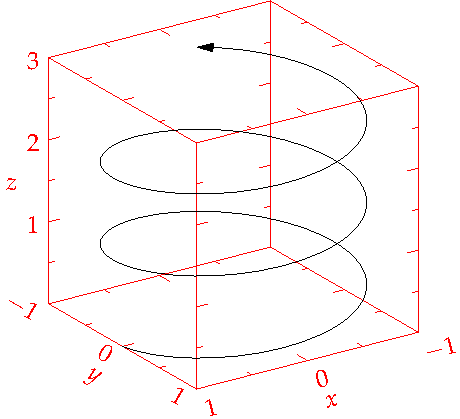
\includegraphics[width=\linewidth]{helix}
\caption{This is a margin figure. The helix is defined by $x = \cos(2\pi z)$, $y = \sin(2\pi z)$, and $z = [0, 2.7]$. The figure was drawn using Asymptote (\url{http://asymptote.sf.net/}).}
\label{fig:marginfig}
\end{marginfigure}

\begin{docspec}
\textbackslash begin\{marginfigure\}\\
\qquad\textbackslash includegraphics\{helix\}\\
\qquad\textbackslash caption\{This is a margin figure.\}\\
\qquad\textbackslash label\{fig:marginfig\}\\
\textbackslash end\{marginfigure\}\\
\end{docspec}

The \docenv{marginfigure} and \docenv{margintable} environments accept an optional parameter \docopt{offset} that adjusts the vertical position of the figure or table. See the ``\nameref{sec:sidenotes}'' section above for examples. The specifications are:
\begin{docspec}
\textbackslash{begin\{marginfigure\}[\docopt{offset}]}\\
\qquad\ldots\\
\textbackslash{end\{marginfigure\}}\\
\mbox{}\\
\textbackslash{begin\{margintable\}[\docopt{offset}]}\\
\qquad\ldots\\
\textbackslash{end\{margintable\}}\\
\end{docspec}

Figure~\ref{fig:fullfig} is an example of the \docenv{figure*} environment and figure~\ref{fig:textfig} is an example of the normal \docenv{figure} environment.

\begin{figure*}[h]
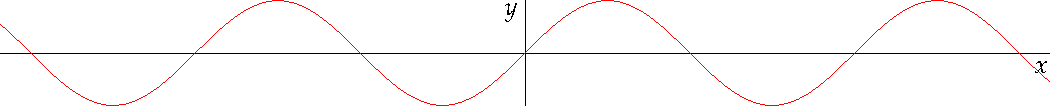
\includegraphics[width=\linewidth]{sine.pdf}
\caption{This graph shows $y = \sin x$ from about $x = [-10, 10]$.
\emph{Notice that this figure takes up the full page width.}}
\label{fig:fullfig}
\end{figure*}

\begin{figure}
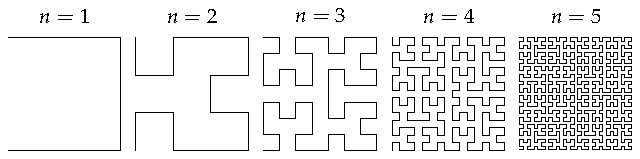
\includegraphics{hilbertcurves.pdf}
\caption[Hilbert curves of various degrees $n$.][6pt]{Hilbert curves of various degrees $n$. \emph{Notice that this figure only takes up the main textblock width.}}
\label{fig:textfig}
\end{figure}

As with sidenotes and marginnotes, a caption may sometimes require vertical adjustment. The \doccmddef{caption} command now takes a second optional argument that enables you to do this by providing a dimension \docopt{offset}. You may specify the caption in any one of the following forms:
\begin{docspec}
\doccmd{caption}\{\docarg{long caption}\}\\
\doccmd{caption}[\docarg{short caption}]\{\docarg{long caption}\}\\
\doccmd{caption}[][\docopt{offset}]\{\docarg{long caption}\}\\
\doccmd{caption}[\docarg{short caption}][\docopt{offset}]%
\{\docarg{long caption}\}
\end{docspec}
A positive \docopt{offset} will push the caption down the page. The short caption, if provided, is what appears in the list of figures/tables, otherwise the ``long'' caption appears there. Note that although the arguments \docopt{short caption} and \docopt{offset} are both optional, they must be provided in order. Thus, to specify an \docopt{offset} without specifying a \docopt{short caption}, you must include the first set of empty brackets \Verb|[]|, which tell \doccmd{caption} to use the default ``long'' caption. As an example, the caption to figure~\ref{fig:textfig} above was given in the form
\begin{docspec}
\doccmd{caption}[Hilbert curves...][6pt]\{Hilbert curves...\}
\end{docspec}

Table~\ref{tab:normaltab} shows table created with the \docpkg{booktabs} package. Notice the lack of vertical rules---they serve only to clutter the table's data.

\begin{table}[ht]
\centering
\fontfamily{ppl}\selectfont
\begin{tabular}{ll}
\toprule
Margin & Length \\
\midrule
Paper width & \unit[8\nicefrac{1}{2}]{inches} \\
Paper height & \unit[11]{inches} \\
Textblock width & \unit[6\nicefrac{1}{2}]{inches} \\
Textblock/sidenote gutter & \unit[\nicefrac{3}{8}]{inches} \\
Sidenote width & \unit[2]{inches} \\
\bottomrule
\end{tabular}
\caption{Here are the dimensions of the various margins used in the Tufte-handout class.}
\label{tab:normaltab}
\end{table}

\newthought{Occasionally} \LaTeX{} will generate an error message:\label{err:too-many-floats}
\begin{docspec}
Error: Too many unprocessed floats
\end{docspec}
\LaTeX{} tries to place floats in the best position on the page. Until it's finished composing the page, however, it won't know where those positions are. If you have a lot of floats on a page (including sidenotes, margin notes, figures, tables, etc.), \LaTeX{} may run out of ``slots'' to keep track of them and will generate the above error.

\LaTeX{} initially allocates 18 slots for storing floats. To work around this limitation, the \TL document classes provide a \doccmddef{morefloats} command that will reserve more slots.

The first time \doccmd{morefloats} is called, it allocates an additional 34 slots. The second time \doccmd{morefloats} is called, it allocates another 26 slots.

The \doccmd{morefloats} command may only be used two times. Calling it a third time will generate an error message. (This is because we can't safely allocate many more floats or \LaTeX{} will run out of memory.)

If, after using the \doccmd{morefloats} command twice, you continue to get the \texttt{Too many unprocessed floats} error, there are a couple things you can do.

The \doccmddef{FloatBarrier} command will immediately process all the floats before typesetting more material. Since \doccmd{FloatBarrier} will start a new paragraph, you should place this command at the beginning or end of a paragraph.

The \doccmddef{clearpage} command will also process the floats before continuing, but instead of starting a new paragraph, it will start a new page.

You can also try moving your floats around a bit: move a figure or table to the next page or reduce the number of sidenotes. (Each sidenote actually uses \emph{two} slots.)

After the floats have placed, \LaTeX{} will mark those slots as unused so they are available for the next page to be composed.

%------------------------------------------------

\section{Captions}
You may notice that the captions are sometimes misaligned. Due to the way \LaTeX's float mechanism works, we can't know for sure where it decided to put a float. Therefore, the \TL document classes provide commands to override the caption position.

\paragraph{Vertical alignment} To override the vertical alignment, use the \doccmd{setfloatalignment} command inside the float environment. For example:

\begin{fullwidth}
\begin{docspec}
\textbackslash begin\{figure\}[btp]\\
\qquad \textbackslash includegraphics\{sinewave\}\\
\qquad \textbackslash caption\{This is an example of a sine wave.\}\\
\qquad \textbackslash label\{fig:sinewave\}\\
\qquad \hlred{\textbackslash setfloatalignment\{b\}\% forces caption to be bottom-aligned}\\
\textbackslash end\{figure\}
\end{docspec}
\end{fullwidth}

\noindent The syntax of the \doccmddef{setfloatalignment} command is:

\begin{docspec}
\doccmd{setfloatalignment}\{\docopt{pos}\}
\end{docspec}

\noindent where \docopt{pos} can be either \texttt{b} for bottom-aligned captions, or \texttt{t} for top-aligned captions.

\paragraph{Horizontal alignment}\label{par:overriding-horizontal}
To override the horizontal alignment, use either the \doccmd{forceversofloat} or the \doccmd{forcerectofloat} command inside of the float environment. For example:

\begin{fullwidth}
\begin{docspec}
\textbackslash begin\{figure\}[btp]\\
\qquad \textbackslash includegraphics\{sinewave\}\\
\qquad \textbackslash caption\{This is an example of a sine wave.\}\\
\qquad \textbackslash label\{fig:sinewave\}\\
\qquad \hlred{\textbackslash forceversofloat\% forces caption to be set to the left of the float}\\
\textbackslash end\{figure\}
\end{docspec}
\end{fullwidth}

The \doccmddef{forceversofloat} command causes the algorithm to assume the float has been placed on a verso page---that is, a page on the left side of a two-page spread. Conversely, the \doccmddef{forcerectofloat} command causes the algorithm to assume the float has been placed on a recto page---that is, a page on the right side of a two-page spread.

%------------------------------------------------

\section{Full-width text blocks}

In addition to the new float types, there is a \docenvdef{fullwidth} environment that stretches across the main text block and the sidenotes area.

\begin{Verbatim}
\begin{fullwidth}
Lorem ipsum dolor sit amet...
\end{fullwidth}
\end{Verbatim}

\begin{fullwidth}
\small\itshape\lipsum[1]
\end{fullwidth}

%------------------------------------------------

\section{Typography}\label{sec:typography}

\subsection{Typefaces}\label{sec:typefaces}\index{typefaces}
If the Palatino, \textsf{Helvetica}, and \texttt{Bera Mono} typefaces are installed, this style will use them automatically. Otherwise, we'll fall back on the Computer Modern typefaces.

\subsection{Letterspacing}\label{sec:letterspacing}
This document class includes two new commands and some improvements on existing commands for letterspacing.

When setting strings of \allcaps{ALL CAPS} or \smallcaps{small caps}, the letter\-spacing---that is, the spacing between the letters---should be increased slightly.\cite{Bringhurst2005} The \doccmddef{allcaps} command has proper letterspacing for strings of \allcaps{FULL CAPITAL LETTERS}, and the \doccmddef{smallcaps} command has letterspacing for \smallcaps{small capital letters}. These commands will also automatically convert the case of the text to upper- or lowercase, respectively.

The \doccmddef{textsc} command has also been redefined to include letterspacing. The case of the \doccmd{textsc} argument is left as is, however. This allows one to use both uppercase and lowercase letters: \textsc{The Initial Letters Of The Words In This Sentence Are Capitalized.}

%------------------------------------------------

\section{Document Class Options}\label{sec:options}

\index{class options|(}
The \doccls{tufte-book} class is based on the \LaTeX\ \doccls{book} document class. Therefore, you can pass any of the typical book options. There are a few options that are specific to the \doccls{tufte-book} document class, however.

The \docclsoptdef{a4paper} option will set the paper size to \smallcaps{A4} instead of the default \smallcaps{US} letter size.

The \docclsoptdef{sfsidenotes} option will set the sidenotes and title block in a \textsf{sans serif} typeface instead of the default roman.

The \docclsoptdef{twoside} option will modify the running heads so that the page number is printed on the outside edge (as opposed to always printing the page number on the right-side edge in \docclsoptdef{oneside} mode). 

The \docclsoptdef{symmetric} option typesets the sidenotes on the outside edge of the page. This is how books are traditionally printed, but is contrary to Tufte's book design which sets the sidenotes on the right side of the page. This option implicitly sets the \docclsopt{twoside} option.

The \docclsoptdef{justified} option sets all the text fully justified (flush left and right). The default is to set the text ragged right. The body text of Tufte's books are set ragged right. This prevents needless hyphenation and makes it easier to read the text in the slightly narrower column.

The \docclsoptdef{bidi} option loads the \docpkg{bidi} package which is used with \tXeLaTeX\ to typeset bi-directional text. Since the \docpkg{bidi} package needs to be loaded before the sidenotes and cite commands are defined, it can't be loaded in the document preamble.

The \docclsoptdef{debug} option causes the \TL classes to output debug information to the log file which is useful in troubleshooting bugs. It will also cause the graphics to be replaced by outlines.

The \docclsoptdef{nofonts} option prevents the \TL classes from automatically loading the Palatino and Helvetica typefaces. You should use this option if you wish to load your own fonts. If you're using \tXeLaTeX, this option is implied (\ie, the Palatino and Helvetica fonts aren't loaded if you use \tXeLaTeX). 

The \docclsoptdef{nols} option inhibits the letterspacing code. The \TL\ classes try to load the appropriate letterspacing package (either pdf\TeX's \docpkg{letterspace} package or the \docpkg{soul} package). If you're using \tXeLaTeX\ with \docpkg{fontenc}, however, you should configure your own letterspacing. 

The \docclsoptdef{notitlepage} option causes \doccmd{maketitle} to generate a title block instead of a title page. The \doccls{book} class defaults to a title page and the \doccls{handout} class defaults to the title block. There is an analogous \docclsoptdef{titlepage} option that forces \doccmd{maketitle} to generate a full title page instead of the title block.

The \docclsoptdef{notoc} option suppresses \TL's custom table of contents (\textsc{toc}) design. The current \textsc{toc} design only shows unnumbered chapter titles; it doesn't show sections or subsections. The \docclsopt{notoc} option will revert to \LaTeX's \textsc{toc} design.

The \docclsoptdef{nohyper} option prevents the \docpkg{hyperref} package from being loaded. The default is to load the \docpkg{hyperref} package and use the \doccmd{title} and \doccmd{author} contents as metadata for the generated \textsc{pdf}.

\index{class options|)}

%----------------------------------------------------------------------------------------
%	CHAPTER 3
%----------------------------------------------------------------------------------------


\backmatter

%----------------------------------------------------------------------------------------
%	BIBLIOGRAPHY
%----------------------------------------------------------------------------------------

\bibliography{bibliography} % Use the bibliography.bib file for the bibliography
\bibliographystyle{plainnat} % Use the plainnat style of referencing

%----------------------------------------------------------------------------------------

\printindex % Print the index at the very end of the document

\end{document}